\subsection{Autopilot}
	\begin{figure}[H]
		\centering
		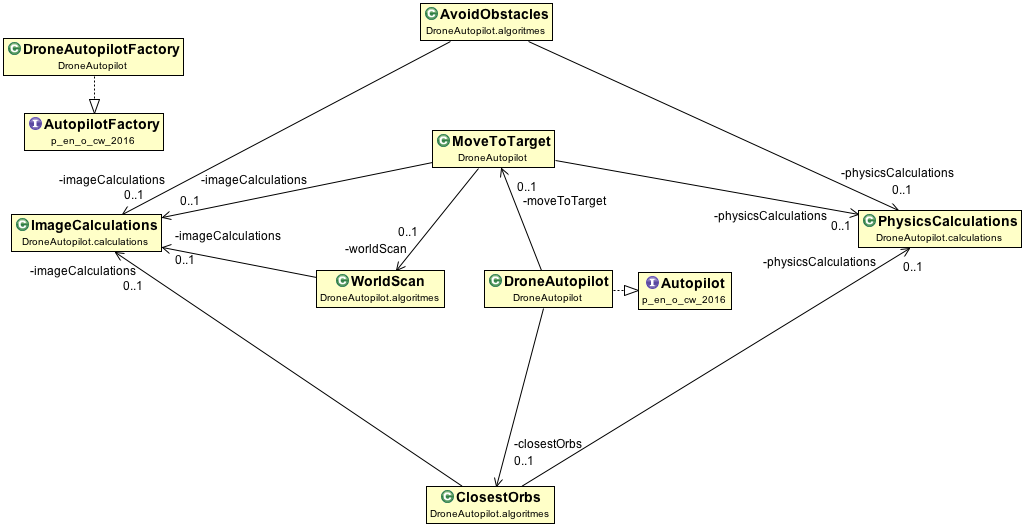
\includegraphics[width=1\textwidth]{AutopilotDiagram.png}
		\caption{Dit klassendiagram geeft de basisstructuur weer van de Autopilot. Ook Figuren \ref{fig: mission} en \ref{fig: control} horen hierin verwerkt te zijn. Echter voor een overzichtelijk beeld van het geheel wordt dit niet gedaan.}
	\end{figure}
	\begin{figure}[H]
		\centering
		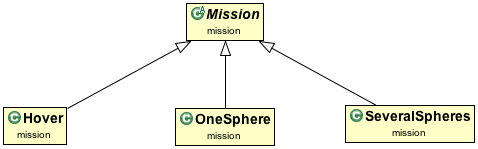
\includegraphics[width=0.6\textwidth]{MissionDiagram.png}
		\caption{Deze figuur geeft de Mission-structuur weer. Deze kan gemakkelijk worden uitgebreid voor extra mijlpalen.}
		\label{fig: mission}
	\end{figure}
	\begin{figure}[H]
		\centering
		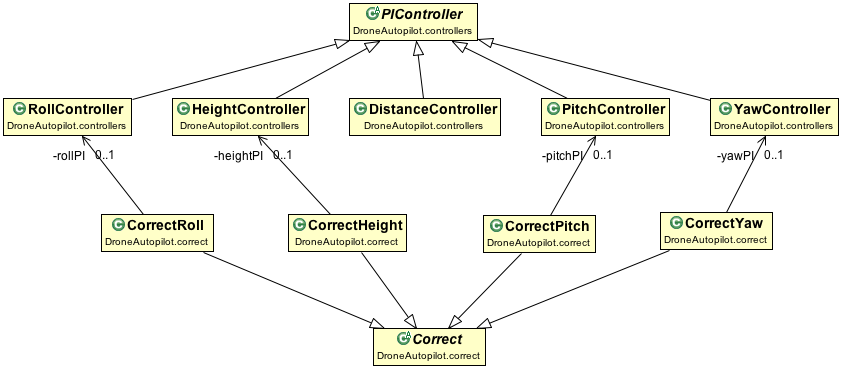
\includegraphics[width=1\textwidth]{ControlDiagram.png}
		\caption{In bovenstaande figuur wordt de controle-eenheid afgebeeld. De \textit{Controllers} geven de wiskundige implementatie weer, terwijl de \textit{Correctors} zorgen voor de correcte implementatie binnen het systeem.}
		\label{fig: control}
	\end{figure}
\subsection{Virtual Testbed}
	\begin{figure}[H]
		\centering
		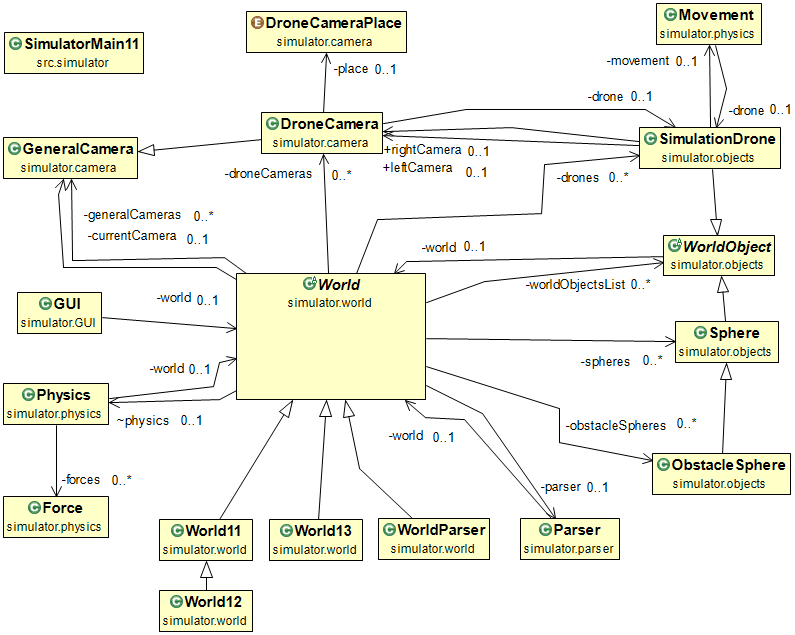
\includegraphics[width=1\textwidth]{Simulator.png}
		\caption{Dit klassendiagram geeft de basisstructuur weer van het Virtual Testbed. Centrale klassen  zijn \textit{World}, \textit{WorldObject} en \textit{GeneralCamera}.}
	\end{figure}